
\thispagestyle{empty}


%kopia zadania BP
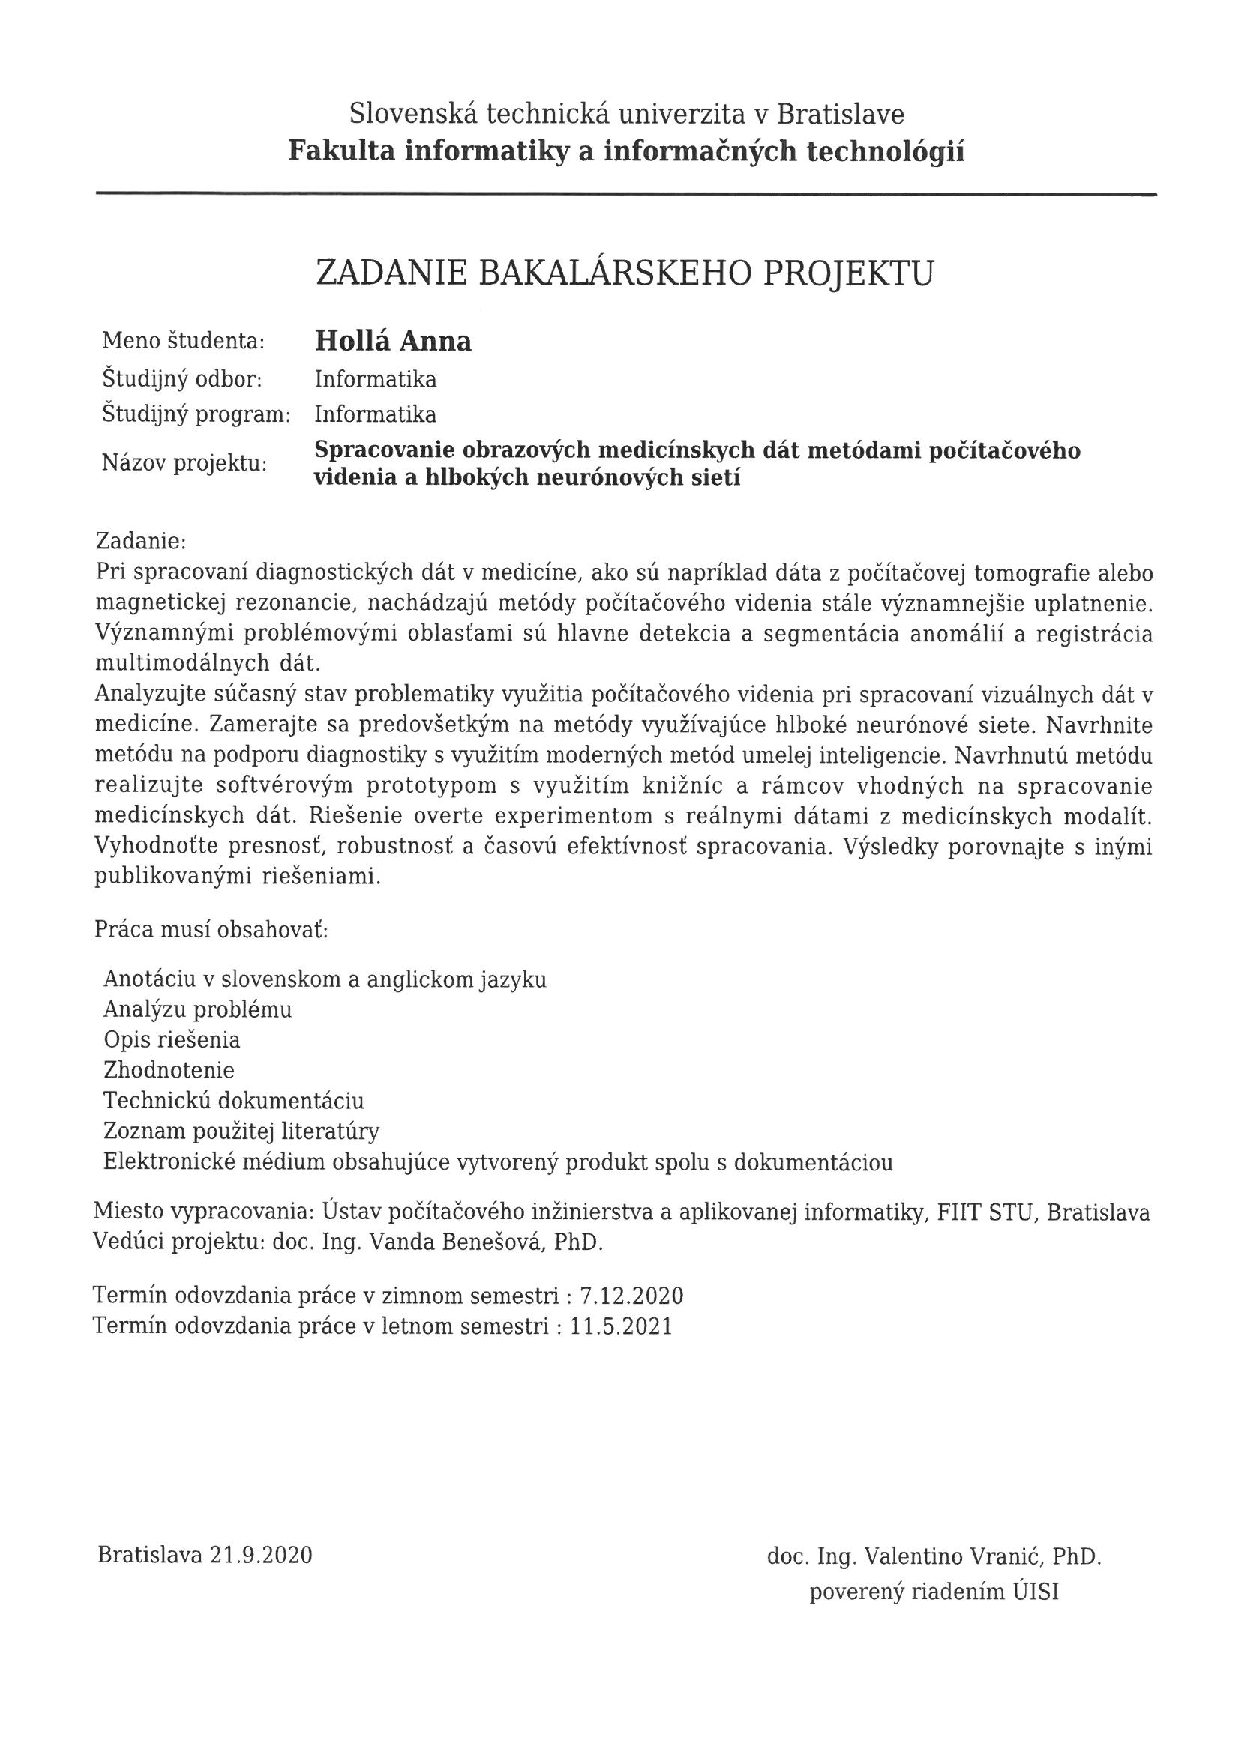
\includepdf[pages={1}]{preamble/zadanieBP_holla.pdf}

\newpage
\thispagestyle{empty}
\mbox{}
\newpage

\thispagestyle{empty}

\section*{Annotation}

\begin{minipage}[t]{1\columnwidth}%

Slovak University of Technology Bratislava 

Faculty of Informatics and Information Technologies



\begin{tabbing}
\hspace{1.5in}     \= \hspace{1in}  \= \hspace{1in}    \kill
Study program:       \> \myStudyProgramENG       \\ 
Author:     \> \myName                  \\
Bachelor Thesis: \> \tabfill{\myTitleENG}   \\
Supervisor:     \> Assoc. Prof. Vanda Benešová  
\end{tabbing}

\myDateENG
\end{minipage}
\\
\\
\\ 
This bachelor thesis addresses the topic of detection and classification of intracranial hemorrhage in non-contrast head CT-scan images. Intracranial hemorrhage is considered a serious and critical health condition, which demands rapid intervention. If not treated instantly, it can have an extremely negative effect on patient's health and in most extreme cases even cause death. Standard approach in diagnosis of this condition is to carry out a CT exam, which is analyzed by radiologists to determine the presence and type of hemorrhage. In the endeavor to provide a tool, which could accelerate and automatize this process, deep learning models, namely neural networks, have shown great performance recently.
\\
In this work, we analyze the given problem and provide the overview of current standard approaches. Based on the conducted research, we propose our own solution, found on deep neural networks and methods of computer vision.



\bigskip{}

\newpage{}\thispagestyle{empty}

\newpage
\thispagestyle{empty}
\mbox{}
\newpage

\thispagestyle{empty}
\section*{Anotácia}

\begin{minipage}[t]{1\columnwidth}%
Slovenská technická univerzita v Bratislave

Fakulta informatiky a informačných technológií


\begin{tabbing}
\hspace{1.5in}     \= \hspace{1in}  \= \hspace{1in}    \kill
Študijný program:       \> \myStudyProgram\\
Autor:     \> \myName                  \\
Bakalárska práca: \> \tabfill{\myTitle}   \\
Vedúci práce: \> \mySupervisor
\end{tabbing}

\myDate
\end{minipage}
\\ \\ \\
Táto bakalárska práca sa zaoberá problematikou detekcie a klasifikácie vnútrolebečného krvácania v bezkontrastných CT snímkoch hlavy. Vnútrolebečné krvácanie je považované za závažný a kritický stav, ktorý si vyžaduje okamžitú medicínsku pomoc. Pri neskorom odhalení môže mať nesmierne negatívny dopad na zdravotný stav pacienta a v extrémnych prípadoch môže skončiť smrťou. Štandardne sú pri podozrení na toto krvácanie pacienti podrobení CT vyšetreniu, ktorého snímky sú pri diagnostike analyzované rádiológmi. V snahe poskytnúť prostriedky, ktoré by urýchlili a zautomatizovali tento proces, sa v poslednej dobe spopularizovalo využitie hlbokých neurónových sietí.
\\
V tejto práci analyzujeme danú problematiku a ponúkame prehľad súčasných štandardných prístupov k riešeniu. Na základe vykonaného prieskumu sme navrhli naše vlastné riešenie, založené na princípe hlbokých neurónových sietí a metódach počítačového videnia.
\bigskip{}




% \newpage{}\thispagestyle{empty}\medskip{}


% \newpage{}

% \newpage
% \thispagestyle{empty}
% \mbox{}
% \newpage

% %kopia zadania BP
% 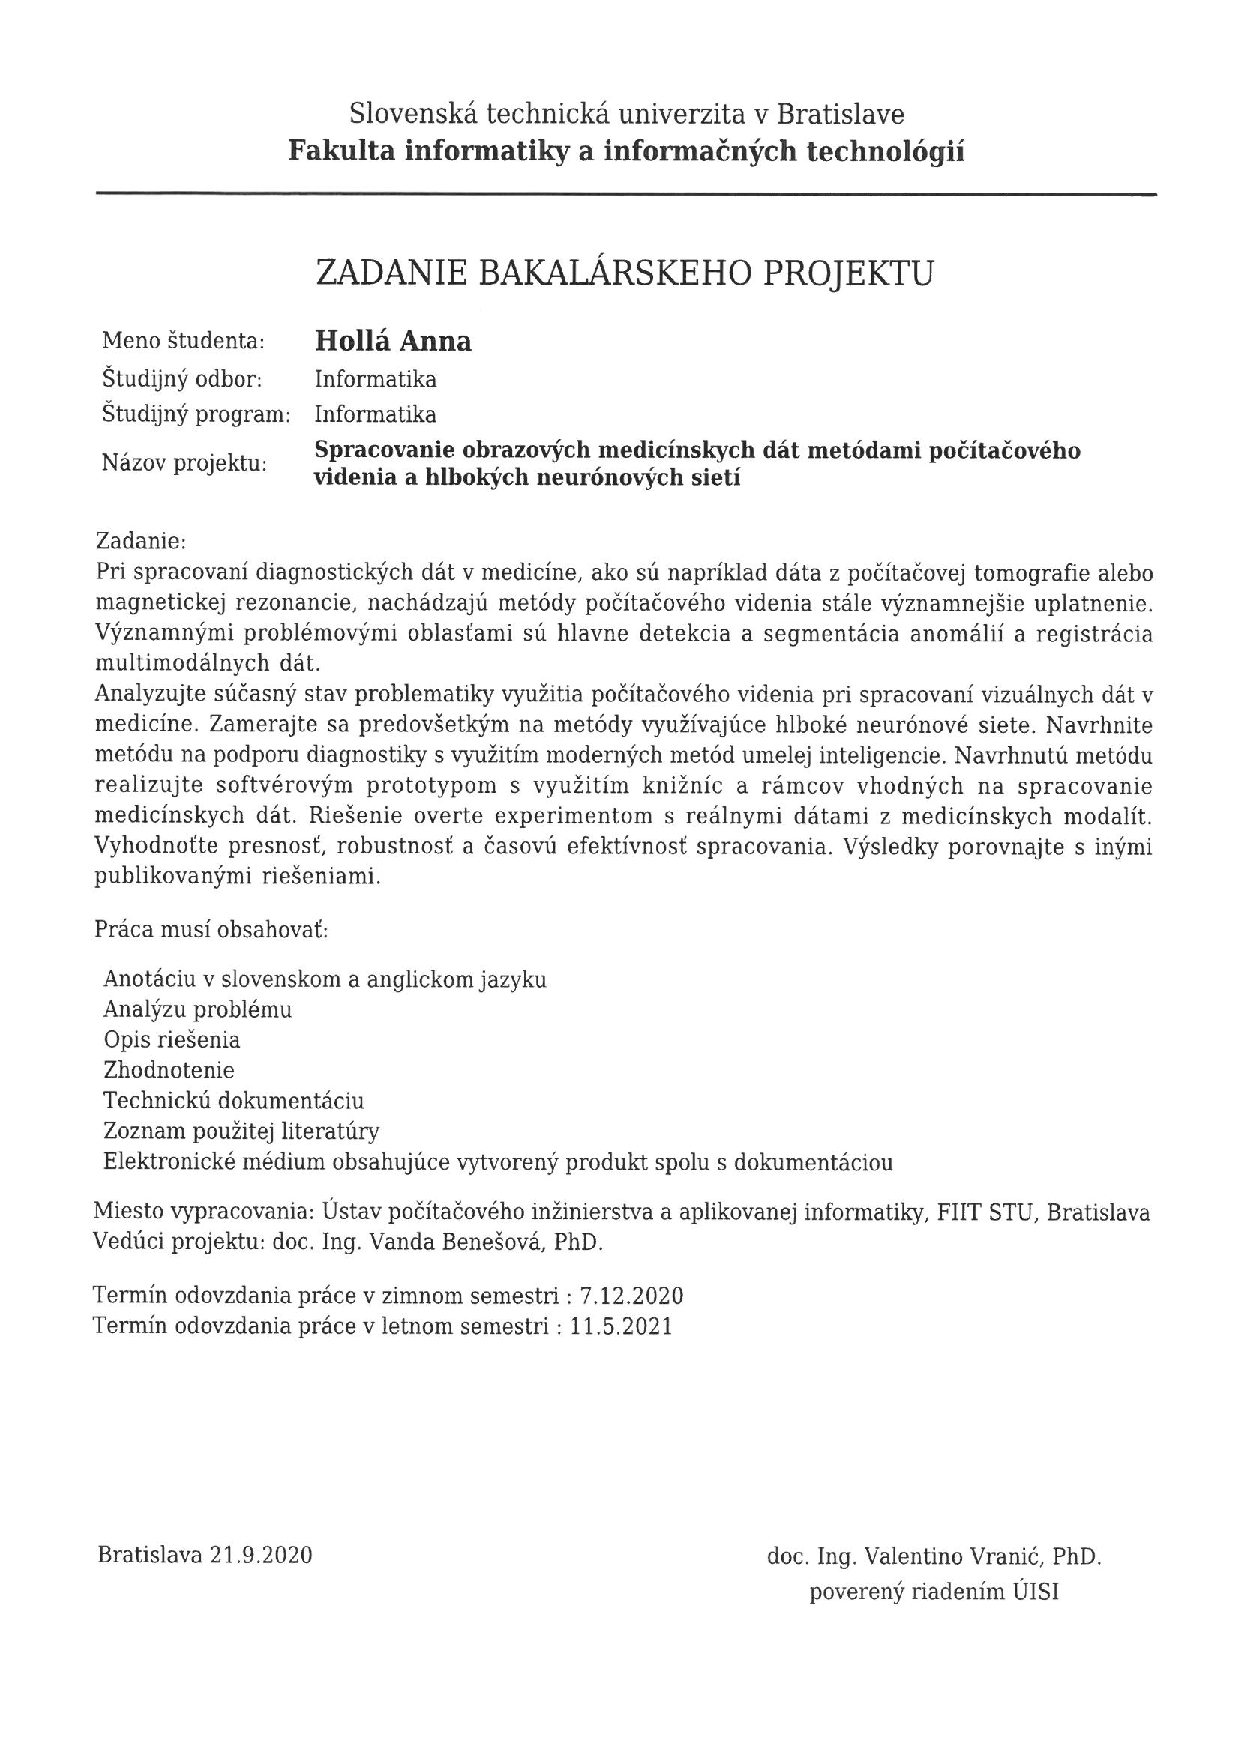
\includepdf[pages={1}]{preamble/zadanieBP_holla.pdf}

\newpage
\thispagestyle{empty}
\mbox{}
\newpage

